\documentclass[]{book}
\usepackage{lmodern}
\usepackage{amssymb,amsmath}
\usepackage{ifxetex,ifluatex}
\usepackage{fixltx2e} % provides \textsubscript
\ifnum 0\ifxetex 1\fi\ifluatex 1\fi=0 % if pdftex
  \usepackage[T1]{fontenc}
  \usepackage[utf8]{inputenc}
\else % if luatex or xelatex
  \ifxetex
    \usepackage{mathspec}
  \else
    \usepackage{fontspec}
  \fi
  \defaultfontfeatures{Ligatures=TeX,Scale=MatchLowercase}
\fi
% use upquote if available, for straight quotes in verbatim environments
\IfFileExists{upquote.sty}{\usepackage{upquote}}{}
% use microtype if available
\IfFileExists{microtype.sty}{%
\usepackage{microtype}
\UseMicrotypeSet[protrusion]{basicmath} % disable protrusion for tt fonts
}{}
\usepackage[margin=1in]{geometry}
\usepackage{hyperref}
\hypersetup{unicode=true,
            pdftitle={Badges in Education},
            pdfauthor={Peter Baumgartner},
            pdfborder={0 0 0},
            breaklinks=true}
\urlstyle{same}  % don't use monospace font for urls
\usepackage{natbib}
\bibliographystyle{apalike}
\usepackage{color}
\usepackage{fancyvrb}
\newcommand{\VerbBar}{|}
\newcommand{\VERB}{\Verb[commandchars=\\\{\}]}
\DefineVerbatimEnvironment{Highlighting}{Verbatim}{commandchars=\\\{\}}
% Add ',fontsize=\small' for more characters per line
\usepackage{framed}
\definecolor{shadecolor}{RGB}{248,248,248}
\newenvironment{Shaded}{\begin{snugshade}}{\end{snugshade}}
\newcommand{\KeywordTok}[1]{\textcolor[rgb]{0.13,0.29,0.53}{\textbf{#1}}}
\newcommand{\DataTypeTok}[1]{\textcolor[rgb]{0.13,0.29,0.53}{#1}}
\newcommand{\DecValTok}[1]{\textcolor[rgb]{0.00,0.00,0.81}{#1}}
\newcommand{\BaseNTok}[1]{\textcolor[rgb]{0.00,0.00,0.81}{#1}}
\newcommand{\FloatTok}[1]{\textcolor[rgb]{0.00,0.00,0.81}{#1}}
\newcommand{\ConstantTok}[1]{\textcolor[rgb]{0.00,0.00,0.00}{#1}}
\newcommand{\CharTok}[1]{\textcolor[rgb]{0.31,0.60,0.02}{#1}}
\newcommand{\SpecialCharTok}[1]{\textcolor[rgb]{0.00,0.00,0.00}{#1}}
\newcommand{\StringTok}[1]{\textcolor[rgb]{0.31,0.60,0.02}{#1}}
\newcommand{\VerbatimStringTok}[1]{\textcolor[rgb]{0.31,0.60,0.02}{#1}}
\newcommand{\SpecialStringTok}[1]{\textcolor[rgb]{0.31,0.60,0.02}{#1}}
\newcommand{\ImportTok}[1]{#1}
\newcommand{\CommentTok}[1]{\textcolor[rgb]{0.56,0.35,0.01}{\textit{#1}}}
\newcommand{\DocumentationTok}[1]{\textcolor[rgb]{0.56,0.35,0.01}{\textbf{\textit{#1}}}}
\newcommand{\AnnotationTok}[1]{\textcolor[rgb]{0.56,0.35,0.01}{\textbf{\textit{#1}}}}
\newcommand{\CommentVarTok}[1]{\textcolor[rgb]{0.56,0.35,0.01}{\textbf{\textit{#1}}}}
\newcommand{\OtherTok}[1]{\textcolor[rgb]{0.56,0.35,0.01}{#1}}
\newcommand{\FunctionTok}[1]{\textcolor[rgb]{0.00,0.00,0.00}{#1}}
\newcommand{\VariableTok}[1]{\textcolor[rgb]{0.00,0.00,0.00}{#1}}
\newcommand{\ControlFlowTok}[1]{\textcolor[rgb]{0.13,0.29,0.53}{\textbf{#1}}}
\newcommand{\OperatorTok}[1]{\textcolor[rgb]{0.81,0.36,0.00}{\textbf{#1}}}
\newcommand{\BuiltInTok}[1]{#1}
\newcommand{\ExtensionTok}[1]{#1}
\newcommand{\PreprocessorTok}[1]{\textcolor[rgb]{0.56,0.35,0.01}{\textit{#1}}}
\newcommand{\AttributeTok}[1]{\textcolor[rgb]{0.77,0.63,0.00}{#1}}
\newcommand{\RegionMarkerTok}[1]{#1}
\newcommand{\InformationTok}[1]{\textcolor[rgb]{0.56,0.35,0.01}{\textbf{\textit{#1}}}}
\newcommand{\WarningTok}[1]{\textcolor[rgb]{0.56,0.35,0.01}{\textbf{\textit{#1}}}}
\newcommand{\AlertTok}[1]{\textcolor[rgb]{0.94,0.16,0.16}{#1}}
\newcommand{\ErrorTok}[1]{\textcolor[rgb]{0.64,0.00,0.00}{\textbf{#1}}}
\newcommand{\NormalTok}[1]{#1}
\usepackage{longtable,booktabs}
\usepackage{graphicx,grffile}
\makeatletter
\def\maxwidth{\ifdim\Gin@nat@width>\linewidth\linewidth\else\Gin@nat@width\fi}
\def\maxheight{\ifdim\Gin@nat@height>\textheight\textheight\else\Gin@nat@height\fi}
\makeatother
% Scale images if necessary, so that they will not overflow the page
% margins by default, and it is still possible to overwrite the defaults
% using explicit options in \includegraphics[width, height, ...]{}
\setkeys{Gin}{width=\maxwidth,height=\maxheight,keepaspectratio}
\IfFileExists{parskip.sty}{%
\usepackage{parskip}
}{% else
\setlength{\parindent}{0pt}
\setlength{\parskip}{6pt plus 2pt minus 1pt}
}
\setlength{\emergencystretch}{3em}  % prevent overfull lines
\providecommand{\tightlist}{%
  \setlength{\itemsep}{0pt}\setlength{\parskip}{0pt}}
\setcounter{secnumdepth}{5}
% Redefines (sub)paragraphs to behave more like sections
\ifx\paragraph\undefined\else
\let\oldparagraph\paragraph
\renewcommand{\paragraph}[1]{\oldparagraph{#1}\mbox{}}
\fi
\ifx\subparagraph\undefined\else
\let\oldsubparagraph\subparagraph
\renewcommand{\subparagraph}[1]{\oldsubparagraph{#1}\mbox{}}
\fi

%%% Use protect on footnotes to avoid problems with footnotes in titles
\let\rmarkdownfootnote\footnote%
\def\footnote{\protect\rmarkdownfootnote}

%%% Change title format to be more compact
\usepackage{titling}

% Create subtitle command for use in maketitle
\newcommand{\subtitle}[1]{
  \posttitle{
    \begin{center}\large#1\end{center}
    }
}

\setlength{\droptitle}{-2em}
  \title{Badges in Education}
  \pretitle{\vspace{\droptitle}\centering\huge}
  \posttitle{\par}
  \author{Peter Baumgartner}
  \preauthor{\centering\large\emph}
  \postauthor{\par}
  \predate{\centering\large\emph}
  \postdate{\par}
  \date{2018-05-30}

\usepackage{booktabs}
\usepackage{booktabs}
\usepackage{longtable}
\usepackage{array}
\usepackage{multirow}
\usepackage[table]{xcolor}
\usepackage{wrapfig}
\usepackage{float}
\usepackage{colortbl}
\usepackage{pdflscape}
\usepackage{tabu}
\usepackage{threeparttable}
\usepackage{threeparttablex}
\usepackage[normalem]{ulem}
\usepackage{makecell}

\usepackage{amsthm}
\newtheorem{theorem}{Theorem}[chapter]
\newtheorem{lemma}{Lemma}[chapter]
\theoremstyle{definition}
\newtheorem{definition}{Definition}[chapter]
\newtheorem{corollary}{Corollary}[chapter]
\newtheorem{proposition}{Proposition}[chapter]
\theoremstyle{definition}
\newtheorem{example}{Example}[chapter]
\theoremstyle{definition}
\newtheorem{exercise}{Exercise}[chapter]
\theoremstyle{remark}
\newtheorem*{remark}{Remark}
\newtheorem*{solution}{Solution}
\begin{document}
\maketitle

{
\setcounter{tocdepth}{1}
\tableofcontents
}
\chapter{Preface}\label{preface}

Still to write

\chapter{Badges in Stack Overflow}\label{badges-in-stack-overflow}

\section{The Stack Exchange Network}\label{the-stack-exchange-network}

\subsection{172 Websites with Stack Overflow as
Showpiece}\label{websites-with-stack-overflow-as-showpiece}

Why I am using Stack Overflow as my primary example to investigate the
usefulness of badges in education?

\href{https://stackoverflow.com/}{Stack Overflow} is a very successful
Question and Answer (Q\&A) website. It hosts the world's largest
programming community and is still growing. Stack Overflow occupies
about the 60th position in the world rankings of websites. Currently
(June 2018) it has 8.9 million registered user with 16 million questions
and 25 million answers. There are already clones in different languages
(Russian , Japanese, Spanish and Portuguese) whose user basis at least
are partially to add.

But Stack Overflow is just the
\href{https://stackexchange.com/sites\#traffic}{flagship of
StackExchange}, a network of (currently) 173 Q\&A websites, following
the same principles for community management. With this high number of
Q\&A websites for different issues and target groups it is allowed to
assume that at least some principles of the successful community
management of programmer are not only restricted to technical subjects
but can be transferred to other areas as well. One can see from the
\href{https://stackexchange.com/sites?view=grid\#}{graphical
represenation} of the Stack Exchange sites that technology, ``hard
sciences'' like mathematics, physics, chemistry dominate the network.
But there are also websites on philosophy, language learning and even
websites addressing recreational issues like bicycles, chess and beer,
wine \& spirits.

\begin{quote}
Stack Exchange network consists of 173 Q\&A communities including Stack
Overflow, the largest, most trusted online community for developers to
learn, share their knowledge, and build their careers. (Quote from the
Stack Overflow website) \footnote{This quote apears in a little window
  when you are on the \href{https://meta.stackexchange.com}{meta site}
  and you click in the StackExchange banner left from the search field.
  But actually in my downloaded data I found just 172 websites. On the
  about site of \href{https://stackexchange.com/about}{StackExchange}
  however I have seen outdated information from the year 2015 (Today:
  25th May 2018). You can find another summary of the astonishing
  success story of StackOverflow from a business perspective on the
  \href{https://stackoverflow.com/company}{company page of
  StackOverflow}. -- It is sometimes difficult for me to find the right
  place for some information because of the complex clutter of (similar)
  sites on different levels (site and meta site).}
\end{quote}

\subsection{\texorpdfstring{``Graduates'' Websites and Websites on Trial
(Beta)}{Graduates Websites and Websites on Trial (Beta)}}\label{graduates-websites-and-websites-on-trial-beta}

\subsection{Stack Exchange Websites by
Subject}\label{stack-exchange-websites-by-subject}

\begin{tabular}{r|l|r}
\hline
Status & Users & \makecell[l]{Rank\\(Users)}\\
\hline
121 & 3D Printing & 14126\\
\hline
32 & Academia & 809172\\
\hline
128 & Amateur Radio & 21229\\
\hline
11 & Android Enthusiasts & 298418\\
\hline
75 & Anime and Manga & 136640\\
\hline
59 & Arduino & 66162\\
\hline
19 & Arqade & 1196579\\
\hline
102 & Artificial Intelligence & 14471\\
\hline
157 & Arts and Crafts & 11021\\
\hline
9 & Ask Different & 712554\\
\hline
111 & Ask Patents & 19535\\
\hline
3 & Ask Ubuntu & 2426259\\
\hline
88 & Astronomy & 78833\\
\hline
171 & Augur & 1970\\
\hline
71 & Aviation & 303072\\
\hline
145 & Beer, Wine and Spirits & 13387\\
\hline
106 & Biblical Hermeneutics & 78541\\
\hline
68 & Bicycles & 178700\\
\hline
161 & Bioinformatics & 11132\\
\hline
65 & Biology & 191516\\
\hline
37 & Bitcoin & 144177\\
\hline
51 & Blender & 216189\\
\hline
82 & Board and Card Games & 152222\\
\hline
132 & Bricks & 35808\\
\hline
130 & Buddhism & 60913\\
\hline
49 & Chemistry & 279218\\
\hline
105 & Chess & 65006\\
\hline
110 & Chinese Language & 57445\\
\hline
78 & Christianity & 221190\\
\hline
152 & CiviCRM & 37720\\
\hline
13 & Code Review & 611983\\
\hline
146 & Coffee & 13426\\
\hline
159 & Community Building & 11899\\
\hline
80 & Computational Science & 64019\\
\hline
136 & Computer Graphics & 18229\\
\hline
31 & Computer Science & 217180\\
\hline
148 & Computer Science Educators & 19698\\
\hline
172 & Constructed Languages & 3932\\
\hline
139 & Craft CMS & 52228\\
\hline
12 & Cross Validated & 786372\\
\hline
46 & Cryptography & 157410\\
\hline
52 & Data Science & 56681\\
\hline
18 & Database Administrators & 469686\\
\hline
134 & DevOps & 13643\\
\hline
41 & Drupal Answers & 404345\\
\hline
126 & Earth Science & 55050\\
\hline
129 & Ebooks & 11175\\
\hline
108 & Economics & 43278\\
\hline
16 & Electrical Engineering & 841553\\
\hline
114 & elementary OS & 21762\\
\hline
101 & Emacs & 92732\\
\hline
95 & Engineering & 42028\\
\hline
8 & English Language and Usage & 1481069\\
\hline
38 & English Language Learners & 385908\\
\hline
170 & Esperanto Language & 20958\\
\hline
56 & Ethereum & 96103\\
\hline
127 & Expatriates & 30806\\
\hline
141 & ExpressionEngine Answers & 38458\\
\hline
96 & Freelancing & 18850\\
\hline
99 & French Language & 94873\\
\hline
24 & Game Development & 398126\\
\hline
112 & Gardening and Landscaping & 121757\\
\hline
149 & Genealogy and Family History & 32442\\
\hline
23 & Geographic Information Systems & 580540\\
\hline
77 & German Language & 179714\\
\hline
27 & Graphic Design & 253721\\
\hline
133 & Hardware Recommendations & 15635\\
\hline
117 & Health & 36456\\
\hline
120 & Hinduism & 84696\\
\hline
79 & History & 223596\\
\hline
138 & History of Science and Mathematics & 24607\\
\hline
39 & Home Improvement & 245460\\
\hline
123 & Homebrewing & 51763\\
\hline
14 & Information Security & 804060\\
\hline
137 & Internet of Things & 15484\\
\hline
92 & Interpersonal Skills & 164404\\
\hline
165 & Iota & 6548\\
\hline
91 & Islam & 91721\\
\hline
153 & Italian Language & 25389\\
\hline
84 & Japanese Language & 190366\\
\hline
135 & Joomla & 29222\\
\hline
167 & Korean Language & 9156\\
\hline
155 & Language Learning & 10815\\
\hline
162 & Latin Language & 33069\\
\hline
103 & Law & 59201\\
\hline
85 & Lifehacks & 48395\\
\hline
109 & Linguistics & 61628\\
\hline
158 & Literature & 29756\\
\hline
45 & Magento & 273336\\
\hline
140 & Martial Arts & 28516\\
\hline
53 & Mathematica & 661322\\
\hline
4 & Mathematics & 5882881\\
\hline
131 & Mathematics Educators & 65536\\
\hline
28 & MathOverflow & 1602182\\
\hline
10 & Meta Stack Exchange & 2359776\\
\hline
119 & Mi Yodeya & 295736\\
\hline
144 & Monero & 28142\\
\hline
67 & Motor Vehicle Maintenance and Repair & 145203\\
\hline
48 & Movies and TV & 419847\\
\hline
142 & Music Fans & 17120\\
\hline
60 & Music: Practice and Theory & 206517\\
\hline
154 & Mythology and Folklore & 22824\\
\hline
57 & Network Engineering & 71390\\
\hline
93 & Open Data & 33657\\
\hline
118 & Open Source & 30408\\
\hline
76 & Parenting & 163702\\
\hline
43 & Personal Finance and Money & 342948\\
\hline
122 & Pets & 52902\\
\hline
70 & Philosophy & 120510\\
\hline
44 & Photography & 323326\\
\hline
81 & Physical Fitness & 83098\\
\hline
15 & Physics & 1070047\\
\hline
151 & Poker & 14869\\
\hline
83 & Politics & 175514\\
\hline
160 & Portuguese Language & 21318\\
\hline
35 & Programming Puzzles and Code Golf & 754859\\
\hline
74 & Project Management & 60146\\
\hline
97 & Psychology and Neuroscience & 54462\\
\hline
55 & Puzzling & 408970\\
\hline
73 & Quantitative Finance & 80685\\
\hline
163 & Quantum Computing & 5532\\
\hline
33 & Raspberry Pi & 132530\\
\hline
143 & Retrocomputing & 44695\\
\hline
86 & Reverse Engineering & 41393\\
\hline
98 & Robotics & 22701\\
\hline
62 & Role-playing Games & 828985\\
\hline
125 & Russian Language & 49644\\
\hline
116 & Russian Language in Russian & 62925\\
\hline
54 & Salesforce & 337324\\
\hline
30 & Science Fiction and Fantasy & 1518543\\
\hline
47 & Seasoned Advice & 303008\\
\hline
5 & Server Fault & 1786115\\
\hline
42 & SharePoint & 250778\\
\hline
66 & Signal Processing & 78147\\
\hline
156 & Sitecore & 36509\\
\hline
64 & Skeptics & 347251\\
\hline
7 & Software Engineering & 2033673\\
\hline
69 & Software Quality Assurance and Testing & 60843\\
\hline
63 & Software Recommendations & 79986\\
\hline
107 & Sound Design & 62622\\
\hline
87 & Space Exploration & 159476\\
\hline
113 & Spanish Language & 72463\\
\hline
124 & Sports & 55733\\
\hline
58 & Stack Apps & 25462\\
\hline
1 & Stack Overflow & 120153708\\
\hline
89 & Stack Overflow in Japanese & 58858\\
\hline
26 & Stack Overflow in Portuguese & 564539\\
\hline
20 & Stack Overflow in Russian & 789319\\
\hline
29 & Stack Overflow in Spanish & 185438\\
\hline
169 & Stellar & 3003\\
\hline
2 & Super User & 2973385\\
\hline
147 & Sustainable Living & 22882\\
\hline
17 & TeX - LaTeX & 1917801\\
\hline
115 & The Great Outdoors & 130856\\
\hline
36 & The Workplace & 928769\\
\hline
61 & Theoretical Computer Science & 210784\\
\hline
100 & Tor & 19978\\
\hline
40 & Travel & 593827\\
\hline
164 & Tridion & 57724\\
\hline
168 & Ukrainian Language & 16335\\
\hline
6 & Unix and Linux & 1415391\\
\hline
25 & User Experience & 442531\\
\hline
166 & Vegetarianism & 8167\\
\hline
90 & Vi and Vim & 59355\\
\hline
94 & Video Production & 36927\\
\hline
21 & Web Applications & 256782\\
\hline
34 & Webmasters & 188325\\
\hline
104 & Windows Phone & 24025\\
\hline
150 & Woodworking & 30348\\
\hline
22 & WordPress Development & 352509\\
\hline
50 & Worldbuilding & 651310\\
\hline
72 & Writing & 116058\\
\hline
\end{tabular}

\section{Dynamics of the Stack Exchange
Community}\label{dynamics-of-the-stack-exchange-community}

But before to look into these other websites one should grasp the
community dynamics of the most successful member of the network.

All Stack Exchange websites are based of a complex interplay between
different elements:

\begin{enumerate}
\def\labelenumi{\arabic{enumi}.}
\tightlist
\item
  \textbf{Scores (``reputation'' points)} are earned through positive
  votes by peers for posting useful answers but also for asking
  questions, if they show research effort and their underlying problems
  are reproducible.
\item
  \textbf{Badges} as digital token in form of emblems. They are awarded
  by the system either for fulfilling certain tasks or reaching a
  certain amount of community awareness.
\item
  \textbf{Priviliges} are granted when certain thresholds or milestones
  of reputation points are transcended. Each privilege opens up a
  specified user rights in relation to the website.
\end{enumerate}

I am convinced that the study of user interactions of Stack Overflow can
be very helpful to understand the success factors for a prosperous
community building process. To study user behavior and their reactions
to the rules and framework of Stack Overflow one can learn not only much
about the effects of gamification elements (e.g.~the interplay between
reputation points and badges) but also how communities of practice work.

Besides the common review of literature my research in this paper is
based on four sources:

\begin{enumerate}
\def\labelenumi{\arabic{enumi}.}
\tightlist
\item
  \textbf{\href{https://stackoverflow.com/}{Stack Overflow}:} Clearly
  enough this has to be one of my chief source of information.
\item
  \textbf{\href{http://api.stackexchange.com/}{Stack Exchance API}:} The
  Stack Exchange network provides an Application Programming Interface
  (API) where one can download data for answering research question.
\item
  \textbf{\href{https://meta.stackoverflow.com/}{Meta Stack Overflow}:}
  This website is especially dedicated to Q\&A \emph{about} Stack
  Overflow itself. The discussion on this website is an important
  resource on qualitative data to my research question.
\item
  \textbf{\href{https://meta.stackexchange.com/}{Meta Stack Exchange}:}
  Another for meta-discussion. This time for the whole Stack Exchange
  family of Q\&A websites, so to speak the meta-meta-website of the
  Stack Overflow website.
\end{enumerate}

\section{Categorization of Badges}\label{categorization-of-badges}

I need to download all types of badges with their description and for
further investigation to categorize them.

\subsection{Badges for different
activities}\label{badges-for-different-activities}

The badges are grouped according to the necessary activities to get
them. The long version what you have to do to get a a specific badge is
posted on meta.stackexchance.com under the title:
\href{https://meta.stackexchange.com/questions/67397/list-of-all-badges-with-full-descriptions}{List
of all badges with full descriptions}. A short and more readable version
can be seen on \href{https://stackoverflow.com/help/badges}{help page
for badges}:

\begin{enumerate}
\def\labelenumi{\arabic{enumi})}
\tightlist
\item
  Question badges
\item
  Answer badges
\item
  Participation badges
\item
  Moderation badges
\item
  Other badges
\item
  Documentation badges
\end{enumerate}

\subsection{Badges from different
sources}\label{badges-from-different-sources}

Another differentiation is the point of origin the badges come from.
Even though all badges are generated automatically by the system, there
are two principal sources to get them. There are two different entities
responsible for awarding badges.

\begin{itemize}
\tightlist
\item
  There are badges you can get by just doing a certain action once or a
  needed number of times. * And there are badges you get only after some
  community action.
\end{itemize}

I call the first type \texttt{user} and the second type \texttt{peer}
badges.

\textbf{Examples for \texttt{user} badges:}

\begin{itemize}
\tightlist
\item
  Name: ``Civic Duty'' (Vote 300 times).
\item
  Name: ``Enthusiast'' (Visit the site each day for 30 consecutive day)
\end{itemize}

Some of the \texttt{user} badges are only available after some threshold
value is reached and a certain privileges is granted. For instance
voting up needs 15 and voting down 125 reputation points.

\textbf{Examples for \texttt{peer} badges:}

\begin{itemize}
\tightlist
\item
  Name: ``Favorite Question'' (Question favored by 25 users)
\item
  Name: ``Popular Question'' (Question with 1000 views).
\end{itemize}

There are also badges tied with certain events, like moderator election,
working with the beta version, meeting employees at an event etc. Mostly
these badges are in my categorization \texttt{user} badges, but you
cannot get them at any time, even if you would have the required
privileges.

The badge system of Stack Overflow is a dynamic system. When the website
was launched (September 15, 2008) it did not start with all 91 badges
which are listed today (May 21, 2018). Some of the badges were added
during the history of the website but other are not awarded anymore.
Some of those badges which are not functional anymore are retired badges
(e.g. ``Analytical'', for visiting all sections of the FAQ). This means
you will still see some veteran users with these badges. Other badges
(all three documentation badges for instance) are withdrawn, e.g.~they
were even deleted from those user accounts they were awarded earlier. I
call these two groups of badges \texttt{event} and \texttt{dead} badges.

To sum up there are 4 points of origin for badges:

\begin{enumerate}
\def\labelenumi{\arabic{enumi})}
\tightlist
\item
  Badges from user action = \texttt{user} badges
\item
  Badges from community action = \texttt{peer} badges
\item
  Badges from some action during a specified occurrence = \texttt{event}
  badges
\item
  Badges where the point of origin is not interesting anymore as they
  are now non-functional = \texttt{dead} badges
\end{enumerate}

\subsection{Badges with different degrees of
difficulty}\label{badges-with-different-degrees-of-difficulty}

Badges are ranked by their difficulty. According to their level of
difficulty users are awarded with bronze (relatively easy), silver
(moderately difficult) or gold (difficult) badges.

There are badges with the same action required but with different amount
of repetition. User can see those groups of badges separated by lines on
the \href{https://stackoverflow.com/help/badges}{Stack Overflow
website}. On this page one can also inspect how many time each badge was
awarded.

There is also a special group of badges intimately linked with
reputation of the user's expertise. These \texttt{Tag\ Badges} also come
with different degrees of difficulty.

I will focus in my research on those badges where users are mainly
responsible. Those are the badges where I can show if users are
motivated to strive for them.

\textbf{Visit the site each day for {[}\ldots{}{]} consecutive days.
(Days are counted in UTC.)}

\begin{itemize}
\tightlist
\item
  30 (Enthusiast)
\item
  100 (Fanatic)
\end{itemize}

\textbf{Ask a well-received question {[}\ldots{}{]} and maintain a
positive question record}

\begin{itemize}
\tightlist
\item
  on 5 separate days (Curious)
\item
  on 30 separate days (Inquisitativ)
\item
  on 100 separate days (Socratic)
\end{itemize}

\textbf{Complete at least {[}\ldots{}{]}. This badge is awarded once per
review type}

\begin{itemize}
\tightlist
\item
  one review task (Custodian)
\item
  250 review tasks (Reviewer)
\item
  1000 review tasks (Steward)
\end{itemize}

\textbf{Edit and answer {[}\ldots{}{]} (both actions within 12 hours,
answer score \textgreater{} 0)}

\begin{itemize}
\tightlist
\item
  1 question (Explainer)
\item
  50 questions (Refiner)
\item
  500 questions (Illuminator)
\end{itemize}

\textbf{Edit}

\begin{itemize}
\tightlist
\item
  first post (Editor)
\item
  80 posts (Strunk \& White)
\item
  500 posts (Copy Editor)
\end{itemize}

\textbf{Edit {[}\ldots{}{]} that was inactive for 6 months}

\begin{itemize}
\tightlist
\item
  first post (Excavator)
\item
  100 posts (Archaeologist)
\end{itemize}

The \texttt{user} badges are of utmost importance for my research. Most
of these badges are granted for quality assurance work on the website
and are not linked with reputation points. They are -- from a systemic
perspective -- important for the dynamic of the website and maintain
respective raise the quality of the platform and their ecological
sustainability.

When I can show that people are striving to get \texttt{user} badges --
even when they are not linked with reputation points -- than it is
evident that badges are some additional (motivational) factors for the
community development.

\begin{landscape}\rowcolors{2}{white}{gray!6}

\begin{longtable}[t]{lr>{\raggedright\arraybackslash}p{2cm}rllll>{\raggedright\arraybackslash}p{9cm}}
\caption{\label{tab:display-badges-table-landscape}Badges in Stack Overflow}\\
\hiderowcolors
\toprule
  & ID & Name & Count & Rank & Activity & Origin & Alike & Description\\
\midrule
\endfirsthead
\caption[]{\label{tab:display-badges-table-landscape}Badges in Stack Overflow \textit{(continued)}}\\
\toprule
  & ID & Name & Count & Rank & Activity & Origin & Alike & Description\\
\midrule
\endhead
\
\endfoot
\bottomrule
\endlastfoot
\showrowcolors
1 & 222 & Altruist & 8158 & bronze & Question & User & XX & First bounty you manually award on another person's question\\
2 & 1306 & Analytical & 43743 & bronze & Other & Dead & XX & Visited every section of the FAQ (retired)\\
3 & 260 & Announcer & 131289 & bronze & Other & Peer & 22 & Share a link to a question later visited by 25 unique IP addresses\\
4 & 1286 & Archaeologist & 1883 & silver & Moderation & User & 20 & Edit 100 posts that were inactive for 6 months\\
5 & 9 & Autobiographer & 799567 & bronze & Participation & User & XX & Complete "About Me" section of user profile\\
\addlinespace
6 & 221 & Benefactor & 38879 & bronze & Question & User & XX & First bounty you manually award on your own question\\
7 & 30 & Beta & 2510 & silver & Participation & Event & 13 & Voted 10 times, added 3 posts score > 0, and visited the site on 3 separate days during the private beta\\
8 & 261 & Booster & 3234 & silver & Other & Peer & 22 & Share a link to a question later visited by 300 unique IP addresses\\
9 & 1973 & Caucus & 573681 & bronze & Participation & Event & 09 & Visit an election during any phase of an active election and have enough reputation to cast a vote\\
10 & 6644 & Census & 71168 & silver & Other & Event & XX & Completed the annual Stack Overflow survey; your responses are anonymous\\
\addlinespace
11 & 8 & Citizen Patrol & 177509 & bronze & Moderation & User & 16 & First flagged post\\
12 & 32 & Civic Duty & 80312 & silver & Moderation & User & XX & Vote 300 or more times\\
13 & 4 & Cleanup & 40887 & bronze & Moderation & User & XX & First rollback\\
14 & 31 & Commentator & 799870 & bronze & Participation & User & 10 & Leave 10 comments\\
15 & 3108 & Constable & 0 & gold & Moderation & Event & 17 & Served as a pro-tem moderator for at least 1 year or through site graduation\\
\addlinespace
16 & 1974 & Constituent & 186464 & silver & Participation & Event & 09 & Vote for a candidate in the final phase of an election\\
17 & 901 & Convention & 2041 & silver & Participation & Peer & 14 & 10 posts with score of 2 on meta\\
18 & 223 & Copy Editor & 2807 & gold & Moderation & User & 19 & Edit 500 posts (excluding own or deleted posts and tag edits)\\
19 & 7 & Critic & 337868 & bronze & Moderation & User & XX & First down vote\\
20 & 4127 & Curious & 283493 & bronze & Question & User & 01 & Ask a well-received question on 5 separate days, and maintain a positive question record\\
\addlinespace
21 & 2278 & Custodian & 660176 & bronze & Moderation & User & 18 & Complete at least one review task. This badge is awarded once per review type\\
22 & 1002 & Deputy & 10655 & silver & Moderation & User & 16 & Raise 80 helpful flags\\
23 & 37 & Disciplined & 10866 & bronze & Moderation & User & XX & Delete own post with score of 3 or higher\\
24 & 6157 & Documentation Beta & 294 & silver & Documentation & Dead & XX & Contributed 3+ substantive pieces of documentation during the private beta\\
25 & 6158 & Documentation Pioneer & 2359 & silver & Documentation & Dead & XX & Contributed 3+ substantive pieces of documentation in the first month of documentation\\
\addlinespace
26 & 7358 & Documentation User & 43292 & silver & Documentation & Dead & XX & Earned at least one badge for contributing to Stack Overflow Documentation\\
27 & 3 & Editor & 1941240 & bronze & Moderation & User & 19 & First edit\\
28 & 155 & Electorate & 17053 & gold & Moderation & User & XX & Vote on 600 questions and 25\% or more of total votes are on questions\\
29 & 19 & Enlightened & 326889 & silver & Answer & Peer & XX & First to answer and accepted with score of 10 or more\\
30 & 71 & Enthusiast & 184881 & silver & Participation & User & 11 & Visit the site each day for 30 consecutive days. (Days are counted in UTC.)\\
\addlinespace
31 & 145 & Epic & 659 & silver & Participation & Peer & 12 & Earn 200 daily reputation 50 times\\
32 & 1287 & Excavator & 116182 & bronze & Moderation & User & 20 & Edit first post that was inactive for 6 months\\
33 & 4368 & Explainer & 55984 & bronze & Answer & User & 05 & Edit and answer 1 question (both actions within 12 hours, answer score > 0)\\
34 & 28 & Famous Question & 531146 & gold & Question & Peer & 04 & Question with 10,000 views\\
35 & 83 & Fanatic & 28042 & gold & Participation & User & 11 & Visit the site each day for 100 consecutive days. (Days are counted in UTC.)\\
\addlinespace
36 & 33 & Favorite Question & 42126 & silver & Question & Peer & 02 & Question favorited by 25 users\\
37 & 15 & Generalist & 1018 & silver & Answer & Peer & XX & Provide non-wiki answers of 15 total score in 20 of top 40 tags\\
38 & 24 & Good Answer & 338757 & silver & Answer & Peer & 06 & Answer score of 25 or more\\
39 & 21 & Good Question & 158537 & silver & Question & Peer & 03 & Question score of 25 or more\\
40 & 25 & Great Answer & 58424 & gold & Answer & Peer & 06 & Answer score of 100 or more\\
\addlinespace
41 & 22 & Great Question & 26490 & gold & Question & Peer & 03 & Question score of 100 or more\\
42 & 18 & Guru & 107423 & silver & Answer & Peer & XX & Accepted answer and score of 40 or more\\
43 & 4370 & Illuminator & 92 & gold & Answer & User & 05 & Edit and answer 500 questions (both actions within 12 hours, answer score > 0)\\
44 & 2600 & Informed & 1728997 & bronze & Other & User & XX & Read the entire tour page\\
45 & 4128 & Inquisitive & 28311 & silver & Question & User & 01 & Ask a well-received question on 30 separate days, and maintain a positive question record\\
\addlinespace
46 & 219 & Investor & 16376 & bronze & Question & User & XX & First bounty you offer on another person's question\\
47 & 146 & Legendary & 250 & gold & Participation & Peer & 12 & Earn 200 daily reputation 150 times\\
48 & 1298 & Marshal & 2512 & gold & Moderation & User & 16 & Raise 500 helpful flags\\
49 & 144 & Mortarboard & 29156 & bronze & Participation & Peer & 12 & Earn at least 200 reputation (the daily maximum) in a single day\\
50 & 17 & Necromancer & 451138 & silver & Answer & Peer & 07 & Answer a question more than 60 days later with score of 5 or more\\
\addlinespace
51 & 23 & Nice Answer & 1020981 & bronze & Answer & Peer & 06 & Answer score of 10 or more\\
52 & 20 & Nice Question & 491031 & bronze & Question & Peer & 03 & Question score of 10 or more\\
53 & 6381 & Not a Robot & 892 & silver & Other & Event & XX & Met a Stack Overflow employee at an event where Stack Overflow was an organizer or participant with 50 or more attendees\\
54 & 27 & Notable Question & 1859667 & silver & Question & Peer & 04 & Question with 2,500 views\\
55 & 5 & Organizer & 111063 & bronze & Moderation & User & XX & First retag\\
\addlinespace
56 & 998 & Outspoken & 1156 & silver & Participation & Peer & 15 & Post 10 messages in chat starred by 10 different users\\
57 & 38 & Peer Pressure & 186488 & bronze & Moderation & User & XX & Delete own post with score of -3 or lower\\
58 & 26 & Popular Question & 3725497 & bronze & Question & Peer & 04 & Question with 1,000 views\\
59 & 62 & Populist & 16770 & gold & Answer & Peer & XX & Highest scoring answer that outscored an accepted answer with score of more than 10 by more than 2x\\
60 & 892 & Precognitive & 0 & bronze & Participation & Dead & 13 & Followed the Area 51 proposal for this site before it entered the commitment phase\\
\addlinespace
61 & 220 & Promoter & 69063 & bronze & Question & User & XX & First bounty you offer on your own question\\
62 & 1276 & Proofreader & 16465 & bronze & Moderation & User & XX & Approve or reject 100 suggested edits\\
63 & 262 & Publicist & 953 & gold & Other & Peer & 22 & Share a link to a question later visited by 1000 unique IP addresses\\
64 & 94 & Pundit & 9207 & silver & Participation & Peer & 10 & Leave 10 comments with score of 5 or more\\
65 & 900 & Quorum & 25227 & bronze & Participation & Peer & 14 & One post with score of 2 on meta\\
\addlinespace
66 & 4369 & Refiner & 1774 & silver & Answer & User & 05 & Edit and answer 50 questions (both actions within 12 hours, answer score > 0)\\
67 & 1656 & Research Assistant & 280 & silver & Moderation & User & 21 & Edit 50 tag wikis\\
68 & 95 & Reversal & 291 & gold & Answer & Peer & XX & Provide an answer of +20 score to a question of -5 score\\
69 & 1478 & Reviewer & 33425 & silver & Moderation & User & 18 & Complete at least 250 review tasks. This badge is awarded once per review type\\
70 & 837 & Revival & 324339 & bronze & Answer & User & 07 & Answer more than 30 days after a question was asked as first answer scoring 2 or more\\
\addlinespace
71 & 10 & Scholar & 1597231 & bronze & Question & User & XX & Ask a question and accept an answer\\
72 & 14 & Self-Learner & 122119 & bronze & Answer & User & XX & Answer your own question with score of 3 or more\\
73 & 3109 & Sheriff & 36 & gold & Moderation & Event & 17 & Served as an elected moderator for at least 1 year\\
74 & 4129 & Socratic & 3362 & gold & Question & User & 01 & Ask a well-received question on 100 separate days, and maintain a positive question record\\
75 & 805 & Sportsmanship & 2572 & silver & Moderation & User & XX & Up vote 100 answers on questions where an answer of yours has a positive score\\
\addlinespace
76 & 36 & Stellar Question & 6046 & gold & Question & Peer & 02 & Question favorited by 100 users\\
77 & 2279 & Steward & 11887 & gold & Moderation & User & 18 & Complete at least 1,000 review tasks. This badge is awarded once per review type\\
78 & 12 & Strunk \&amp; White & 14705 & silver & Moderation & User & 19 & Edit 80 posts\\
79 & 2 & Student & 1937383 & bronze & Question & User & XX & First question with score of 1 or more\\
80 & 804 & Suffrage & 43785 & bronze & Moderation & User & XX & Use 30 votes in a day\\
\addlinespace
81 & 6 & Supporter & 1168643 & bronze & Moderation & User & XX & First up vote\\
82 & 1224 & Synonymizer & 899 & bronze & Moderation & Peer & XX & First approved tag synonym\\
83 & 254 & Tag Editor & 21974 & bronze & Moderation & User & 21 & First tag wiki edit\\
84 & 884 & Talkative & 9613 & bronze & Participation & Peer & 15 & Post 10 messages, with 1 or more starred, in chat\\
85 & 11 & Taxonomist & 11747 & silver & Moderation & Peer & XX & Create a tag used by 50 questions\\
\addlinespace
86 & 1 & Teacher & 1266655 & bronze & Answer & User & XX & Answer a question with score of 1 or more\\
87 & 225 & Tenacious & 48183 & silver & Answer & User & 08 & Zero score accepted answers: more than 5 and 20\% of total\\
88 & 63 & Tumbleweed & 998633 & bronze & Question & Peer & XX & Asked a question with zero score, no answers, no comments, and low views for a week\\
89 & 226 & Unsung Hero & 18860 & gold & Answer & Peer & 08 & Zero score accepted answers: more than 10 and 25\% of total\\
90 & 1108 & Vox Populi & 28464 & bronze & Moderation & User & XX & Use the maximum 40 votes in a day\\
91 & 13 & Yearling & 1329469 & silver & Participation & Event & XX & Active member for a year, earning at least 200 reputation\\*
\end{longtable}
\rowcolors{2}{white}{white}
\end{landscape}

\chapter{Introduction}\label{intro}

Still to write

\chapter{Methods}\label{methods}

We describe our methods in this chapter.

\chapter{Applications}\label{applications}

Some \emph{significant} applications are demonstrated in this chapter.

\section{Example one}\label{example-one}

\section{Example two}\label{example-two}

\chapter{Final Words}\label{final-words}

We have finished a nice book.

\chapter{Appendix}\label{appendix}

\section{Material from original bookdown
files}\label{material-from-original-bookdown-files}

\subsection{Prerequisites}\label{prerequisites}

This is a \emph{sample} book written in \textbf{Markdown}. You can use
anything that Pandoc's Markdown supports, e.g., a math equation
\(a^2 + b^2 = c^2\).

The \textbf{bookdown} package can be installed from CRAN or Github:

\begin{Shaded}
\begin{Highlighting}[]
\OperatorTok{>}\StringTok{ }\KeywordTok{install.packages}\NormalTok{(}\StringTok{"bookdown"}\NormalTok{)}
\OperatorTok{>}\StringTok{ }\CommentTok{# or the development version}
\ErrorTok{>}\StringTok{ }\CommentTok{# devtools::install_github("rstudio/bookdown")}
\end{Highlighting}
\end{Shaded}

Remember each Rmd file contains one and only one chapter, and a chapter
is defined by the first-level heading \texttt{\#}.

To compile this example to PDF, you need XeLaTeX. You are recommended to
install TinyTeX (which includes XeLaTeX):
\url{https://yihui.name/tinytex/}.

\subsection{Intro of the minimal book
example}\label{intro-of-the-minimal-book-example}

You can label chapter and section titles using \texttt{\{\#label\}}
after them, e.g., we can reference Chapter \ref{intro}. If you do not
manually label them, there will be automatic labels anyway, e.g.,
Chapter \ref{methods}.

Figures and tables with captions will be placed in \texttt{figure} and
\texttt{table} environments, respectively.

\begin{Shaded}
\begin{Highlighting}[]
\OperatorTok{>}\StringTok{ }\KeywordTok{par}\NormalTok{(}\DataTypeTok{mar =} \KeywordTok{c}\NormalTok{(}\DecValTok{4}\NormalTok{, }\DecValTok{4}\NormalTok{, .}\DecValTok{1}\NormalTok{, .}\DecValTok{1}\NormalTok{))}
\OperatorTok{>}\StringTok{ }\KeywordTok{plot}\NormalTok{(pressure, }\DataTypeTok{type =} \StringTok{'b'}\NormalTok{, }\DataTypeTok{pch =} \DecValTok{19}\NormalTok{)}
\end{Highlighting}
\end{Shaded}

\begin{figure}

{\centering 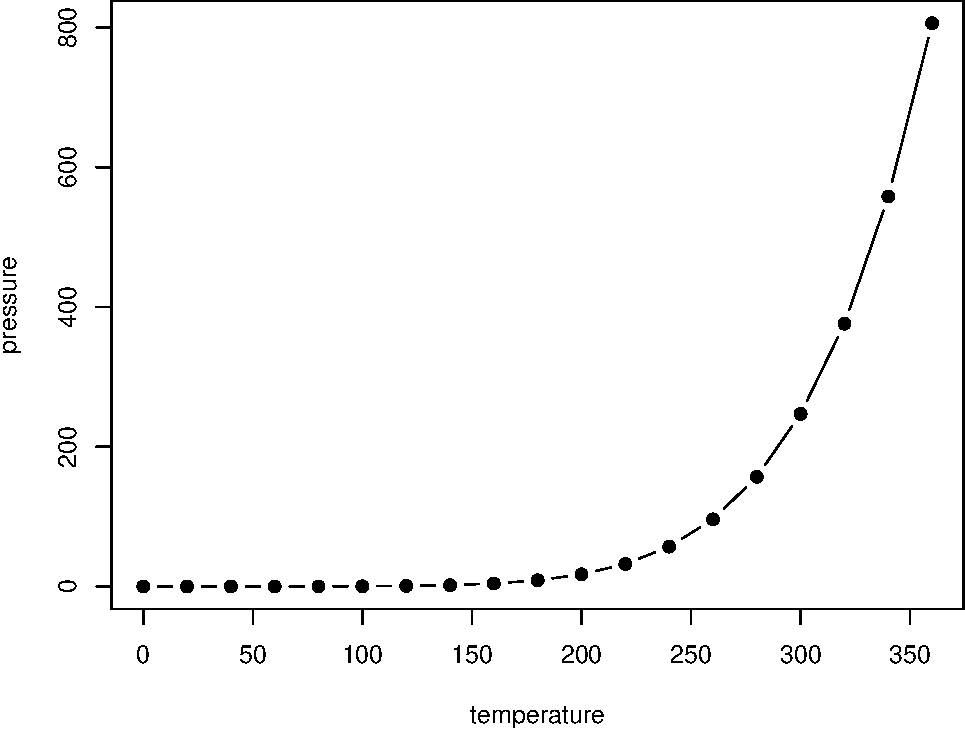
\includegraphics[width=0.8\linewidth]{badges4edu_files/figure-latex/nice-fig-1} 

}

\caption{Here is a nice figure!}\label{fig:nice-fig}
\end{figure}

Reference a figure by its code chunk label with the \texttt{fig:}
prefix, e.g., see Figure \ref{fig:nice-fig}. Similarly, you can
reference tables generated from \texttt{knitr::kable()}, e.g., see Table
\ref{tab:nice-tab}.

\begin{Shaded}
\begin{Highlighting}[]
\OperatorTok{>}\StringTok{ }\NormalTok{knitr}\OperatorTok{::}\KeywordTok{kable}\NormalTok{(}
\OperatorTok{+}\StringTok{   }\KeywordTok{head}\NormalTok{(iris, }\DecValTok{20}\NormalTok{), }\DataTypeTok{caption =} \StringTok{'Here is a nice table!'}\NormalTok{,}
\OperatorTok{+}\StringTok{   }\DataTypeTok{booktabs =} \OtherTok{TRUE}
\OperatorTok{+}\StringTok{ }\NormalTok{)}
\end{Highlighting}
\end{Shaded}

\begin{table}

\caption{\label{tab:nice-tab}Here is a nice table!}
\centering
\begin{tabular}[t]{rrrrl}
\toprule
Sepal.Length & Sepal.Width & Petal.Length & Petal.Width & Species\\
\midrule
5.1 & 3.5 & 1.4 & 0.2 & setosa\\
4.9 & 3.0 & 1.4 & 0.2 & setosa\\
4.7 & 3.2 & 1.3 & 0.2 & setosa\\
4.6 & 3.1 & 1.5 & 0.2 & setosa\\
5.0 & 3.6 & 1.4 & 0.2 & setosa\\
\addlinespace
5.4 & 3.9 & 1.7 & 0.4 & setosa\\
4.6 & 3.4 & 1.4 & 0.3 & setosa\\
5.0 & 3.4 & 1.5 & 0.2 & setosa\\
4.4 & 2.9 & 1.4 & 0.2 & setosa\\
4.9 & 3.1 & 1.5 & 0.1 & setosa\\
\addlinespace
5.4 & 3.7 & 1.5 & 0.2 & setosa\\
4.8 & 3.4 & 1.6 & 0.2 & setosa\\
4.8 & 3.0 & 1.4 & 0.1 & setosa\\
4.3 & 3.0 & 1.1 & 0.1 & setosa\\
5.8 & 4.0 & 1.2 & 0.2 & setosa\\
\addlinespace
5.7 & 4.4 & 1.5 & 0.4 & setosa\\
5.4 & 3.9 & 1.3 & 0.4 & setosa\\
5.1 & 3.5 & 1.4 & 0.3 & setosa\\
5.7 & 3.8 & 1.7 & 0.3 & setosa\\
5.1 & 3.8 & 1.5 & 0.3 & setosa\\
\bottomrule
\end{tabular}
\end{table}

You can write citations, too. For example, we are using the
\textbf{bookdown} package \citep{R-bookdown} in this sample book, which
was built on top of R Markdown and \textbf{knitr} \citep{xie2015}.

\section{My own (miscellanous) tests}\label{my-own-miscellanous-tests}

\subsection{Install stackr with
vignettes}\label{install-stackr-with-vignettes}

Building vignettes takes some time. So if you are in a hurry, than just
install stackr. You can still look at the vignettes in R help. The
difference is: With \texttt{build\_vignettes\ =\ TRUE} and then
\texttt{browseVignettes("stackr")} you can look at the vignettes in your
default browser. This is slightly more comfortable.

\begin{Shaded}
\begin{Highlighting}[]
\OperatorTok{>}\StringTok{ }\NormalTok{devtools}\OperatorTok{::}\KeywordTok{install_github}\NormalTok{(}\StringTok{"dgrtwo/stackr"}\NormalTok{, }\DataTypeTok{build_vignettes =} \OtherTok{TRUE}\NormalTok{)}
\OperatorTok{>}\StringTok{ }\KeywordTok{browseVignettes}\NormalTok{(}\StringTok{"stackr"}\NormalTok{)}
\end{Highlighting}
\end{Shaded}

\section{Load several packages at
once}\label{load-several-packages-at-once}

The following code is part of a debate at SO with different suggestions.
It seems to me, that all suggestions (utility packages, code examples)
has some disadvantages:

\begin{itemize}
\tightlist
\item
  \textbf{lapply:} For me the
  \href{https://stackoverflow.com/questions/8175912/load-multiple-packages-at-once}{best}
  approach -- it uses just \texttt{lapply}. I have changed
  \texttt{require} to \texttt{library} because of the arguments by
  \href{https://yihui.name/en/2014/07/library-vs-require/}{Yihui}. My
  lines now gives a error message and stops if one of the called
  packages is not installed.
\item
  \textbf{easypackages:} is not available on CRAN anymore, has very poor
  downloads.
\item
  \textbf{pacman:} a very sophisticated programm, but -- for me at least
  -- to complex and therefore to much overhead.
\item
  \textbf{installed.packages:}
  \href{https://gist.github.com/stevenworthington/3178163}{ipak.R} This
  loads \emph{and} installs missing packages. It is quite similar as
  \texttt{lappy}-version, but -- because of the if-condition -- more
  complex. Additionally it is checking which packages are installed:
\end{itemize}

\begin{quote}
``This can be slow when thousands of packages are installed, so do not
use this to find out if a named package is installed (use system.file or
find.package) nor to find out if a package is usable (call require and
check the return value) \ldots{}''
\end{quote}

So maybe the best would be to combine the \texttt{lapply} with the
\texttt{installled.packages} version. But insted to use
\texttt{installled.packages} I should use in the if-statement
\texttt{require}, check for the return value and -- if necessary -- to
install missing packages.

\begin{Shaded}
\begin{Highlighting}[]
\OperatorTok{>}\StringTok{ }\NormalTok{x <-}\StringTok{ }\KeywordTok{c}\NormalTok{(}\StringTok{"plyr"}\NormalTok{, }\StringTok{"psych"}\NormalTok{, }\StringTok{"tm"}\NormalTok{)}
\OperatorTok{>}\StringTok{ }\KeywordTok{lapply}\NormalTok{(x, library, }\DataTypeTok{character.only =} \OtherTok{TRUE}\NormalTok{)}
\end{Highlighting}
\end{Shaded}

\subsection{How many downloads of a defined
packages?}\label{how-many-downloads-of-a-defined-packages}

\begin{Shaded}
\begin{Highlighting}[]
\OperatorTok{>}\StringTok{ }\KeywordTok{library}\NormalTok{(dlstats)}
\OperatorTok{>}\StringTok{ }\NormalTok{y <-}\StringTok{ }\KeywordTok{cran_stats}\NormalTok{(}\StringTok{"learnr"}\NormalTok{)}
\OperatorTok{>}\StringTok{ }\KeywordTok{ggplot}\NormalTok{(y, }\KeywordTok{aes}\NormalTok{(start, downloads, }\DataTypeTok{group =}\NormalTok{ package, }\DataTypeTok{color =}\NormalTok{ package)) }\OperatorTok{+}
\OperatorTok{+}\StringTok{         }\KeywordTok{geom_line}\NormalTok{() }\OperatorTok{+}\StringTok{ }\KeywordTok{geom_point}\NormalTok{(}\KeywordTok{aes}\NormalTok{(}\DataTypeTok{shape =}\NormalTok{ package))}
\OperatorTok{>}\StringTok{ }\CommentTok{# cranApp()}
\end{Highlighting}
\end{Shaded}

\section{Some data to remind}\label{some-data-to-remind}

\begin{enumerate}
\def\labelenumi{\arabic{enumi}.}
\tightlist
\item
  How to find answers tagged with \texttt{r} and not active since 6
  month:
  \href{https://stackoverflow.com/search?q=\%5Br\%5D+lastactive\%3A..6m+is\%3Aa}{Search}
\end{enumerate}

\begin{enumerate}
\def\labelenumi{\arabic{enumi}.}
\setcounter{enumi}{2}
\tightlist
\item
  What kind of actions are are allowed with \texttt{combine\_url}?
\end{enumerate}

I have added \texttt{timeline} to the list!

\subsection{Some experiments}\label{some-experiments}

\begin{Shaded}
\begin{Highlighting}[]
\OperatorTok{>}\StringTok{ }\KeywordTok{library}\NormalTok{(tidyverse)}
\OperatorTok{>}\StringTok{ }\KeywordTok{library}\NormalTok{(lubridate)}
\OperatorTok{>}\StringTok{ }\KeywordTok{library}\NormalTok{(jsonlite)}
\OperatorTok{>}\StringTok{ }
\ErrorTok{>}\StringTok{ }\CommentTok{# returns: "Error in open.connection(con, "rb") : HTTP error 400."}
\ErrorTok{>}\StringTok{ }
\ErrorTok{>}\StringTok{ }\NormalTok{json_file1 <-}\StringTok{ "https://api.stackexchange.com/2.2/events?site=stackoverflow&key=mRTYimh499J3lInIGjcxfA(("}
\OperatorTok{>}\StringTok{ }\NormalTok{json_list1 <-}\StringTok{ }\NormalTok{jsonlite}\OperatorTok{::}\KeywordTok{fromJSON}\NormalTok{(json_file1, }\DataTypeTok{flatten =} \OtherTok{TRUE}\NormalTok{)}
\OperatorTok{>}\StringTok{ }\NormalTok{df1 <-}\StringTok{ }\KeywordTok{as.tibble}\NormalTok{(json_list1[[}\DecValTok{1}\NormalTok{]])}
\OperatorTok{>}\StringTok{ }\NormalTok{df1 <-}\StringTok{ }\NormalTok{df1 }\OperatorTok\StringTok{ }\KeywordTok{mutate}\NormalTok{(}\DataTypeTok{created =} \KeywordTok{with_tz}\NormalTok{(}\KeywordTok{as.POSIXct}\NormalTok{(creation_date, }\DataTypeTok{origin =} \StringTok{"1970-01-01"}\NormalTok{), }\StringTok{"UTC"}\NormalTok{))}
\end{Highlighting}
\end{Shaded}

\begin{Shaded}
\begin{Highlighting}[]
\OperatorTok{>}\StringTok{ }\KeywordTok{library}\NormalTok{(dplyr)}
\OperatorTok{>}\StringTok{ }\NormalTok{mtcars[}\DecValTok{1}\OperatorTok{:}\DecValTok{10}\NormalTok{, }\DecValTok{1}\OperatorTok{:}\DecValTok{2}\NormalTok{] }\OperatorTok
\OperatorTok{+}\StringTok{     }\KeywordTok{mutate}\NormalTok{(}
\OperatorTok{+}\StringTok{         }\DataTypeTok{car =} \KeywordTok{row.names}\NormalTok{(.),}
\OperatorTok{+}\StringTok{         }\CommentTok{# You don't need format = "latex" if you have ever defined options(knitr.table.format)}
\OperatorTok{+}\StringTok{         }\DataTypeTok{mpg =} \KeywordTok{cell_spec}\NormalTok{(mpg, }\StringTok{"latex"}\NormalTok{, }\DataTypeTok{color =} \KeywordTok{ifelse}\NormalTok{(mpg }\OperatorTok{>}\StringTok{ }\DecValTok{20}\NormalTok{, }\StringTok{"red"}\NormalTok{, }\StringTok{"blue"}\NormalTok{)),}
\OperatorTok{+}\StringTok{         }\DataTypeTok{cyl =} \KeywordTok{cell_spec}\NormalTok{(cyl, }\StringTok{"latex"}\NormalTok{, }\DataTypeTok{color =} \StringTok{"white"}\NormalTok{, }\DataTypeTok{align =} \StringTok{"c"}\NormalTok{, }\DataTypeTok{angle =} \DecValTok{45}\NormalTok{,}
\OperatorTok{+}\StringTok{             }\DataTypeTok{background =} \KeywordTok{factor}\NormalTok{(cyl, }\KeywordTok{c}\NormalTok{(}\DecValTok{4}\NormalTok{, }\DecValTok{6}\NormalTok{, }\DecValTok{8}\NormalTok{), }\KeywordTok{c}\NormalTok{(}\StringTok{"#666666"}\NormalTok{, }\StringTok{"#999999"}\NormalTok{, }\StringTok{"#BBBBBB"}\NormalTok{)))}
\OperatorTok{+}\StringTok{ }\NormalTok{) }\OperatorTok
\OperatorTok{+}\StringTok{ }\KeywordTok{select}\NormalTok{(car, mpg, cyl) }\OperatorTok
\OperatorTok{+}\StringTok{ }\KeywordTok{kable}\NormalTok{(}\StringTok{"latex"}\NormalTok{, }\DataTypeTok{escape =}\NormalTok{ F, }\DataTypeTok{booktabs =}\NormalTok{ T, }\DataTypeTok{linesep =} \StringTok{""}\NormalTok{)}
\end{Highlighting}
\end{Shaded}

\begin{tabular}{lll}
\toprule
car & mpg & cyl\\
\midrule
Mazda RX4 & \textcolor{red}{21} & \multicolumn{1}{c}{\rotatebox{45}{\cellcolor[HTML]{999999}{\textcolor{white}{6}}}}\\
Mazda RX4 Wag & \textcolor{red}{21} & \multicolumn{1}{c}{\rotatebox{45}{\cellcolor[HTML]{999999}{\textcolor{white}{6}}}}\\
Datsun 710 & \textcolor{red}{22.8} & \multicolumn{1}{c}{\rotatebox{45}{\cellcolor[HTML]{666666}{\textcolor{white}{4}}}}\\
Hornet 4 Drive & \textcolor{red}{21.4} & \multicolumn{1}{c}{\rotatebox{45}{\cellcolor[HTML]{999999}{\textcolor{white}{6}}}}\\
Hornet Sportabout & \textcolor{blue}{18.7} & \multicolumn{1}{c}{\rotatebox{45}{\cellcolor[HTML]{BBBBBB}{\textcolor{white}{8}}}}\\
Valiant & \textcolor{blue}{18.1} & \multicolumn{1}{c}{\rotatebox{45}{\cellcolor[HTML]{999999}{\textcolor{white}{6}}}}\\
Duster 360 & \textcolor{blue}{14.3} & \multicolumn{1}{c}{\rotatebox{45}{\cellcolor[HTML]{BBBBBB}{\textcolor{white}{8}}}}\\
Merc 240D & \textcolor{red}{24.4} & \multicolumn{1}{c}{\rotatebox{45}{\cellcolor[HTML]{666666}{\textcolor{white}{4}}}}\\
Merc 230 & \textcolor{red}{22.8} & \multicolumn{1}{c}{\rotatebox{45}{\cellcolor[HTML]{666666}{\textcolor{white}{4}}}}\\
Merc 280 & \textcolor{blue}{19.2} & \multicolumn{1}{c}{\rotatebox{45}{\cellcolor[HTML]{999999}{\textcolor{white}{6}}}}\\
\bottomrule
\end{tabular}

\begin{Shaded}
\begin{Highlighting}[]
\OperatorTok{>}\StringTok{ }\KeywordTok{library}\NormalTok{(knitr)}
\OperatorTok{>}\StringTok{ }\KeywordTok{library}\NormalTok{(kableExtra)}
\OperatorTok{>}\StringTok{ }\KeywordTok{library}\NormalTok{(tidyverse)}
\OperatorTok{>}\StringTok{ }\NormalTok{dt_lb <-}\StringTok{ }\KeywordTok{as_tibble}\NormalTok{(}\KeywordTok{data.frame}\NormalTok{(}
\OperatorTok{+}\StringTok{     }\DataTypeTok{Item =} \KeywordTok{c}\NormalTok{(}\StringTok{"Hello}\CharTok{\textbackslash{}n}\StringTok{World"}\NormalTok{, }\StringTok{"This}\CharTok{\textbackslash{}n}\StringTok{is a cat"}\NormalTok{),}
\OperatorTok{+}\StringTok{     }\DataTypeTok{Value =} \KeywordTok{c}\NormalTok{(}\DecValTok{10}\NormalTok{, }\DecValTok{100}\NormalTok{),}
\OperatorTok{+}\StringTok{     }\DataTypeTok{Third =} \KeywordTok{c}\NormalTok{(}\StringTok{"xx}\CharTok{\textbackslash{}n}\StringTok{xx"}\NormalTok{, }\StringTok{"yyyy"}\NormalTok{) }\CommentTok{# does not work without linebreak!!!}
\OperatorTok{+}\StringTok{ }\NormalTok{))}
\OperatorTok{>}\StringTok{ }
\ErrorTok{>}\StringTok{ }
\ErrorTok{>}\StringTok{ }
\ErrorTok{>}\StringTok{ }\NormalTok{dt_lb }\OperatorTok
\OperatorTok{+}\StringTok{     }\KeywordTok{mutate_all}\NormalTok{(linebreak) }\OperatorTok\StringTok{ }\CommentTok{# to keep the hard linebreaks in the text items}
\OperatorTok{+}\StringTok{     }\KeywordTok{kable}\NormalTok{(}\DataTypeTok{booktabs =}\NormalTok{ T, }\DataTypeTok{escape =}\NormalTok{ F,}
\OperatorTok{+}\StringTok{     }\DataTypeTok{col.names =} \KeywordTok{linebreak}\NormalTok{(}\KeywordTok{c}\NormalTok{(}\StringTok{"xxxy}\CharTok{\textbackslash{}n}\StringTok{(Name)"}\NormalTok{, }\StringTok{"zzzy}\CharTok{\textbackslash{}n}\StringTok{(Number)"}\NormalTok{, }\StringTok{"Another}\CharTok{\textbackslash{}n}\StringTok{(Name)"}\NormalTok{)))}
\end{Highlighting}
\end{Shaded}

\begin{tabular}{lrl}
\toprule
\makecell[l]{xxxy\\(Name)} & \makecell[l]{zzzy\\(Number)} & \makecell[l]{Another\\(Name)}\\
\midrule
\makecell[l]{Hello\\World} & 10 & \makecell[l]{xx\\xx}\\
\makecell[l]{This\\is a cat} & 100 & 2\\
\bottomrule
\end{tabular}

\subsection{\texorpdfstring{Problems with \texttt{\&} in cell text with
linebreak}{Problems with \& in cell text with linebreak}}\label{problems-with-in-cell-text-with-linebreak}

see \href{https://github.com/haozhu233/kableExtra/issues/207}{github
issue}

\begin{Shaded}
\begin{Highlighting}[]
\OperatorTok{>}\StringTok{ }\KeywordTok{library}\NormalTok{(knitr)}
\OperatorTok{>}\StringTok{ }\KeywordTok{library}\NormalTok{(kableExtra)}
\OperatorTok{>}\StringTok{ }\NormalTok{dt_lb <-}\StringTok{ }\KeywordTok{data.frame}\NormalTok{(}
\OperatorTok{+}\StringTok{     }\DataTypeTok{Item =} \KeywordTok{c}\NormalTok{(}\StringTok{"Hello}\CharTok{\textbackslash{}n}\StringTok{World"}\NormalTok{, }\StringTok{"This & is}\CharTok{\textbackslash{}n}\StringTok{a cat"}\NormalTok{), }\CommentTok{# & generates error}
\OperatorTok{+}\StringTok{     }\DataTypeTok{Value =} \KeywordTok{c}\NormalTok{(}\DecValTok{10}\NormalTok{, }\DecValTok{100}\NormalTok{)}
\OperatorTok{+}\StringTok{ }\NormalTok{)}
\OperatorTok{>}\StringTok{ }
\ErrorTok{>}\StringTok{ }
\ErrorTok{>}\StringTok{ }
\ErrorTok{>}\StringTok{ }\NormalTok{dt_lb }\OperatorTok
\OperatorTok{+}\StringTok{     }\KeywordTok{mutate_all}\NormalTok{(linebreak) }\OperatorTok
\OperatorTok{+}\StringTok{     }\KeywordTok{kable}\NormalTok{(}\DataTypeTok{booktabs =}\NormalTok{ T, }\DataTypeTok{escape =}\NormalTok{ F,}
\OperatorTok{+}\StringTok{     }\DataTypeTok{col.names =} \KeywordTok{linebreak}\NormalTok{(}\KeywordTok{c}\NormalTok{(}\StringTok{"Item}\CharTok{\textbackslash{}n}\StringTok{(Name)"}\NormalTok{, }\StringTok{"Value}\CharTok{\textbackslash{}n}\StringTok{(Number)"}\NormalTok{)))}
\end{Highlighting}
\end{Shaded}

\begin{Shaded}
\begin{Highlighting}[]
\OperatorTok{>}\StringTok{ }\KeywordTok{library}\NormalTok{(knitr)}
\OperatorTok{>}\StringTok{ }\KeywordTok{library}\NormalTok{(kableExtra)}
\OperatorTok{>}\StringTok{ }
\ErrorTok{>}\StringTok{ }\NormalTok{test <-}\StringTok{ }\KeywordTok{head}\NormalTok{(mtcars, }\DataTypeTok{head =} \DecValTok{10}\NormalTok{)}
\OperatorTok{>}\StringTok{ }\NormalTok{test <-}\StringTok{ }\NormalTok{test[, }\KeywordTok{c}\NormalTok{(}\DecValTok{1}\OperatorTok{:}\DecValTok{6}\NormalTok{)]}
\OperatorTok{>}\StringTok{ }
\ErrorTok{>}\StringTok{ }\NormalTok{p <-}\StringTok{ }\KeywordTok{kable}\NormalTok{(test) }\OperatorTok
\OperatorTok{+}\StringTok{   }\KeywordTok{add_header_above}\NormalTok{(}\KeywordTok{c}\NormalTok{(}\StringTok{" "}\NormalTok{ =}\StringTok{ }\DecValTok{1}\NormalTok{, }\StringTok{"Group 1"}\NormalTok{ =}\StringTok{ }\DecValTok{3}\NormalTok{, }\StringTok{"Group 2"}\NormalTok{ =}\StringTok{ }\DecValTok{3}\NormalTok{))}
\OperatorTok{>}\StringTok{ }\NormalTok{p}
\end{Highlighting}
\end{Shaded}

\begin{tabular}{l|r|r|r|r|r|r}
\hline
\multicolumn{1}{c|}{ } & \multicolumn{3}{|c|}{Group 1} & \multicolumn{3}{|c}{Group 2} \\
\cline{2-4} \cline{5-7}
  & mpg & cyl & disp & hp & drat & wt\\
\hline
Mazda RX4 & 21.0 & 6 & 160 & 110 & 3.90 & 2.620\\
\hline
Mazda RX4 Wag & 21.0 & 6 & 160 & 110 & 3.90 & 2.875\\
\hline
Datsun 710 & 22.8 & 4 & 108 & 93 & 3.85 & 2.320\\
\hline
Hornet 4 Drive & 21.4 & 6 & 258 & 110 & 3.08 & 3.215\\
\hline
Hornet Sportabout & 18.7 & 8 & 360 & 175 & 3.15 & 3.440\\
\hline
Valiant & 18.1 & 6 & 225 & 105 & 2.76 & 3.460\\
\hline
\end{tabular}

\bibliography{book.bib,packages.bib}


\end{document}
